\documentclass[cs4size,a4paper,10pt]{ctexart}   

\linespread{1.5}
\usepackage{geometry}%用于设置上下左右页边距
	\geometry{left=2.5cm,right=2.5cm,top=3.2cm,bottom=2.7cm}
\usepackage{xeCJK,amsmath,paralist,enumerate,booktabs,multirow,graphicx,subfig,setspace,listings,lastpage,hyperref}
\usepackage{amsthm, amssymb, bm, color, framed, graphicx, hyperref, mathrsfs}
\usepackage{mathrsfs}  
	\setlength{\parindent}{2em}
	\lstset{language=Matlab}%
\usepackage{fancyhdr}
\usepackage{graphicx}
\usepackage{subfloat}
\usepackage{listings}
\usepackage{xcolor}
\usepackage{float}
\usepackage{paralist}
\usepackage{setspace}
\usepackage{titlesec}
\usepackage{enumitem}
\usepackage{hyperref}
\usepackage{multirow}
\usepackage{threeparttable}
\usepackage{autobreak}
\usepackage{multicol}
\usepackage{subfig}
\usepackage{unicode-math}

\hypersetup{
	colorlinks=true,
	linkcolor=black,
	urlcolor=black
}

\setenumerate{partopsep=0pt,topsep=0pt}
\setitemize{itemsep=0pt,partopsep=0pt,topsep=0pt}

\titlespacing*{\section}{0pt}{3pt}{3pt}
\titlespacing*{\subsection}{0pt}{2pt}{2pt}
\titlespacing*{\subsubsection}{0pt}{1pt}{1pt}
\titlespacing*{\paragraph}{0pt}{0pt}{0pt}

\ctexset{secnumdepth=4,tocdepth=4}
\setlength{\parindent}{0pt}
\setstretch{1.2}


\setCJKmainfont[BoldFont={FZHei-B01},ItalicFont={FZKai-Z03}]{FZShuSong-Z01} 
\setCJKsansfont[BoldFont={FZHei-B01}]{FZKai-Z03} 
\setCJKmonofont[BoldFont={FZHei-B01}]{FZFangSong-Z02}
\setCJKfamilyfont{zhsong}{FZShuSong-Z01} 
\setCJKfamilyfont{zhhei}{FZHei-B01} 
\setCJKfamilyfont{zhkai}[BoldFont={FZHei-B01}]{FZKai-Z03} 
\setCJKfamilyfont{zhfs}[BoldFont={FZHei-B01}]{FZFangSong-Z02} 
\renewcommand*{\songti}{\CJKfamily{zhsong}} 
\renewcommand*{\heiti}{\CJKfamily{zhhei}} 
\renewcommand*{\kaishu}{\CJKfamily{zhkai}} 
\renewcommand*{\fangsong}{\CJKfamily{zhfs}}


\definecolor{mKeyword}{RGB}{0,0,255}          % bule
\definecolor{mString}{RGB}{160,32,240}        % purple
\definecolor{mComment}{RGB}{34,139,34}        % green
\definecolor{mNumber}{RGB}{128,128,128} 

\lstdefinestyle {njulisting} {
	basewidth = 0.5 em,
	lineskip = 3 pt,
	basicstyle = \small\ttfamily,
	% keywordstyle = \bfseries,
	commentstyle = \itshape\color{gray}, 
	basicstyle=\small\ttfamily,
	keywordstyle={\color{mKeyword}},     % sets color for keywords
	stringstyle={\color{mString}},       % sets color for strings
	commentstyle={\color{mComment}},     % sets color for comments
	numberstyle=\tiny\color{mNumber},
	numbers = left,
	captionpos = t,
	breaklines = true,
	xleftmargin = 2 em,
	xrightmargin = 2 em,
	frame=tlrb,
	tabsize=4
}

\lstset{
style = njulisting, % 调用上述样式 
flexiblecolumns % 允许调整字符宽度
}


%================= 基本格式预置 ===========================
\usepackage{fancyhdr}
\pagestyle{fancy}
\lhead{数据管理基础}
\rhead{关系数据库}
\cfoot{\thepage}
\renewcommand{\headrulewidth}{0.4pt}
\renewcommand{\theenumi}{(\arabic{enumi})}
\CTEXsetup[format={\bfseries\zihao{-3}}]{section}
\CTEXsetup[format={\bfseries\zihao{4}}]{subsection}
\CTEXsetup[format={\bfseries\zihao{-4}}]{subsubsection}


\renewcommand{\contentsname}{目录}  
\begin{document}

	\begin{center}
		{\huge\textbf{第二章\ 关系数据库}}
	\end{center}
	%---------目录---------% 
	\pagenumbering{Roman}
	\tableofcontents
	\clearpage

 	%---------正文---------% 
	\pagenumbering{arabic}
	\setcounter{page}{1}
	\setlength{\parskip}{0.65em}

	\setlength\abovedisplayskip{5pt}
	\setlength\belowdisplayskip{5pt}

	\section{关系数据结构及形式化定义}

\subsection{关系}
\begin{itemize}
    \item \textbf{域:}域是一组具有相同数据类型的值的集合
    \item \textbf{笛卡尔积:}给定一组域 $D_1,D_2,\cdots, D_n$,允许其中某些域是相同的,$D_1,D_2,\cdots, D_n$​的笛卡尔积为
    $$D_1\times D_2\times \cdots \times D_n=\{(d_1,d_2,\cdots,d_n) | d_i\in D_i, \,  i= 1,2,\cdots ,n\}$$
    \begin{itemize}
        \item 其中,每一个元素$(d_1,d_2,\cdots,d_n)$叫作一个$n$ \textbf{元组},或简称元组
        \item 元素中的每一个值 $d_i$ 叫做一个\textbf{分量}
        \item 一个域允许的不同取值个数称为这个域的\textbf{基数}
        \item 若 $D_i(i=1,2,\cdots,n)$ 为有限集,其基数为 $m_i(i=1,2,\cdots, n)$ ,则$D_1\times D_2\times \cdots \times D_n$的基数 $M=\displaystyle{\prod_{i=1}^n}m_i$
    \end{itemize}
    \item \textbf{关系:}$D_1\times D_2\times \cdots \times D_n$ 的子集叫做在域名$D_1\times D_2\times \cdots \times D_n$ 上的关系,表示为$R(D_1\times D_2\times \cdots \times D_n)$ 
    \begin{itemize}
        \item $R$ 表示关系的名字
        \item $n$ 是关系的\textbf{目}或者\textbf{度}
    \end{itemize}
    \item 若关系中的某一属性组的值能唯一地标识一个元组,则称该属性组为\textbf{候选码}
    \begin{itemize}
        \item 若一个关系有多个候选码,则选定其中一个为\textbf{主码}
        \item 候选码的诸属性称为\textbf{主属性}
        \item 不包含在任何侯选码中的属性称为\textbf{非主属性}或\textbf{非码属性}
        \item 在简单的情况下,候选码只包含一个属性;在最极端的情况下,关系模式的所有属性组是这个关系模式的候选码,称为\textbf{全码}
    \end{itemize}
    \item 关系可以有三种类型:\textbf{基本关系}(基本表或基表)、\textbf{查询表}和\textbf{视图表}
    \begin{itemize}
        \item 基本关系是实际存在的表,是实际存储数据的逻辑表示
        \item 查询表是查询结果对应的表
        \item 视图表是由基本表或其他视图表导出的表,是虚表,不对应实际存储的数据
    \end{itemize}
    \item 基本关系的性质:
    \begin{itemize}
        \item 列是同质的,即每一列中的分量是同一类型的数据,来自同一个域
        \item 不同的列可出自同一个域,称其中的每一列称为一个属性,不同的属性要给予不同的属性名
        \item 列的顺序无所谓
        \item 任意两个元组的候选码不能相同
        \item 行的顺序无所谓
        \item 分量必须取原子值
    \end{itemize}
\end{itemize}

\subsection{关系模式}
\begin{itemize}
    \item 关系模式是对关系的描述,关系模式是型,关系是值
    \item 关系的描述称为\textbf{关系模式}。可以形式化地表示为 $R(U,D,DOM,F)$
    \begin{itemize}
        \item $R$ 为关系名
        \item $U$ 为组成该关系的属性名集合
        \item $D$ 为 $U$ 中属性所来自的域
        \item $DOM$ 为属性向域的映像集合
        \item $F$ 为属性间数据的依赖关系集合
    \end{itemize}
\end{itemize}

\subsection{关系数据库}
\begin{itemize}
    \item 在一个给定的应用领域中,所有关系的集合构成一个关系数据库
    \item 关系数据库的型,也称关系数据库模式,是对关系数据库的描述
    \item 关系数据库的值,是这些关系模式在某一时刻对应的关系的集合,通常就称为关系数据库
\end{itemize}

\section{关系的完整性}
\begin{itemize}
    \item 实体完整性和参照完整性
    \begin{itemize}
        \item 关系模型必须满足的完整性约束条件称为关系的两个不变性,应该由关系系统自动支持
    \end{itemize}
    \item 用户定义的完整性
    \item 应用领域需要遵循的约束条件,体现了具体领域中的语义约束
\end{itemize}

\subsection{实体完整性}
\begin{itemize}
    \item \textbf{实体完整性规则:}若属性 $A$ 是基本关系 $R$ 的主属性,则属性 $A$ 不能取空值。空值就是“不知道”或“不存在”或“无意义”的值
    \item 对于实体完整性规则的说明:
    \begin{enumerate}[label=\arabic*.]
        \item 实体完整性规则是针对基本关系而言的。一个基本表通常对应现实世界的一个实体集
        \item 现实世界中的实体是可区分的,即它们具有某种唯一性标识
        \item 关系模型中以主码作为唯一性标识
        \item 主码中的属性即主属性不能取空值。主属性取空值,就说明存在某个不可标识的实体,即存在不可区分的实体,这与第2点相矛盾,因此这个规则称为实体完整性
    \end{enumerate}
\end{itemize}

\subsection{参照完整性}
\begin{itemize}
    \item 在关系模型中实体及实体间的联系都是用关系来描述的,自然存在着关系与关系间的引用
    \item 设 $F$ 是基本关系 $R$ 的一个或一组属性,但不是关系 $R$ 的码,$K_s$ 是基本关系 $S$ 的主码。如果 $F$ 与 $K_s$ 相对应,则称 $F$ 是 $R$ 的\textbf{外码},并称基本关系 $R$ 为\textbf{参照关系},基本关系 $S$ 为\textbf{被参照关系}或\textbf{目标关系}
    \begin{itemize}
        \item 其中关系 $R$ 和 $S$ 不一定是不同的关系
        \item 目标关系 $S$ 的主码 $K_s$ 和参照关系的外码 $F$ 必须定义在同一个(或一组)域上
        \item 外码并不一定要与相应的主码同名
        \begin{itemize}
            \item 当外码与相应的主码属于不同关系时,往往取相同的名字,以便于识别
        \end{itemize}
    \end{itemize}
    \begin{figure}[H]
        \vspace{-0.5em}
	    \centering
	    
\includegraphics[width=0.35\textwidth]{images/2.2.2}
        \vspace{-1em}
	\end{figure}
    \item \textbf{参照完整性规则:}若属性(或属性组)$F$ 是基本关系 $R$ 的外码它与基本关系 $S$ 的主码 $K_s$ 相对应(基本关系 $R$ 和 $S$ 不一定是不同的关系),则对于 $R$ 中每个元组在 $F$ 上的值必须为:
    \begin{itemize}
        \item 或者取空值($F$ 的每个属性值均为空值)
        \item 或者等于 $S$ 中某个元组的主码值
    \end{itemize}
\end{itemize}

\subsection{用户定义的完整性}
\begin{itemize}
    \item 用户定义的完整性是针对某一具体关系数据库的约束条件,反映某一具体应用所涉及的数据必须满足的语义要求
    \item 关系模型应提供定义和检验这类完整性的机制,以便用统一的系统的方法处理它们,而不需由应用程序承担这一功能
\end{itemize}

\section{关系代数}

\subsection{传统的集合运算}
\begin{itemize}
    \item 并:$R\cup S = \{t|t\in R \vee t\in S\}$
    \item 差:$R - S = \{t|t\in R \wedge  t\notin S\}$
    \item 交:$R\cap S = \{t|t\in R \wedge  t\in S\}$
    \item 笛卡尔积:$R\times S = \{\overset{\frown}{t_rt_s} |t_r\in R \wedge  t_s \in S\}$
\end{itemize}

\subsection{专门的关系运算}
首先引入几个记号:
\begin{itemize}
    \item $R$,$t\in R$,$t[A_i]$:
    \begin{itemize}
        \item 设关系模式为 $R(A_1,A_2,\cdots, A_n)$
        \item 它的一个关系设为 $R$
        \item $t \in R$表示 $t$ 是 $R$ 的一个元组
        \item $t[A_i]$ 则表示元组 $t$ 中相应于属性 $A_i$的一个分量
    \end{itemize}
    \item $A$,$t[A]$, $A$
    \begin{itemize}
        \item 若$A=\{A_{i1},A_{i_2},\cdots ,A_{ik}\}$,其中 $A_{i1},A_{i_2},\cdots ,A_{ik}$ 是 $A_1,A_2,\cdots, A_n$中的一部分,则 $A$ 称为属性列或属性组
        \item $t[A]=(t[A_{i1}],t[A_{i2}],\cdots ,t[A_{ik}])$表示元组 $t$ 在属性列 $A$上诸分量的集合
        \item $A$ 则表示 $\{A_1,A_2,\cdots, A_n\}$ 中去掉 $\{A_{i1},A_{i_2},\cdots ,A_{ik}\}$ 后剩余的属性组
    \end{itemize}
    \item $\overset{\frown}{t_rt_s}$:
    \begin{itemize}
        \item $R$ 为 $n$ 目关系,$S$ 为 $m$ 目关系
        \item $t_r\in R, t_s \in S,\overset{\frown}{t_rt_s}$ 称为元组的连接
        \item $\overset{\frown}{t_rt_s}$ 是一个 $n + m$ 列的元组,前 $n$ 个分量为 $R$ 中的一个 $n$ 元组,后 $m$ 个分量为 $S$ 中的一个 $m$ 元组
    \end{itemize}
    \item 象集$Z_X$
    \begin{itemize}
        \item 给定一个关系 $R(X,Z)$,$X$ 和 $Z$ 为属性组
        \item 当 $t[X] = x$时,$x$ 在 $R$ 中的象集为:$Z_X = \{t[Z] | t\in R ,t[X] = x\}$
        \item 它表示 $R$ 中属性组 $X$ 上值为 $x$ 的诸元组在 $Z$ 上分量的集合 
    \end{itemize}
\end{itemize}

下例中的学生—课程数据库如下:
\begin{figure}[H]
    \vspace{-0.5em}
	\centering
	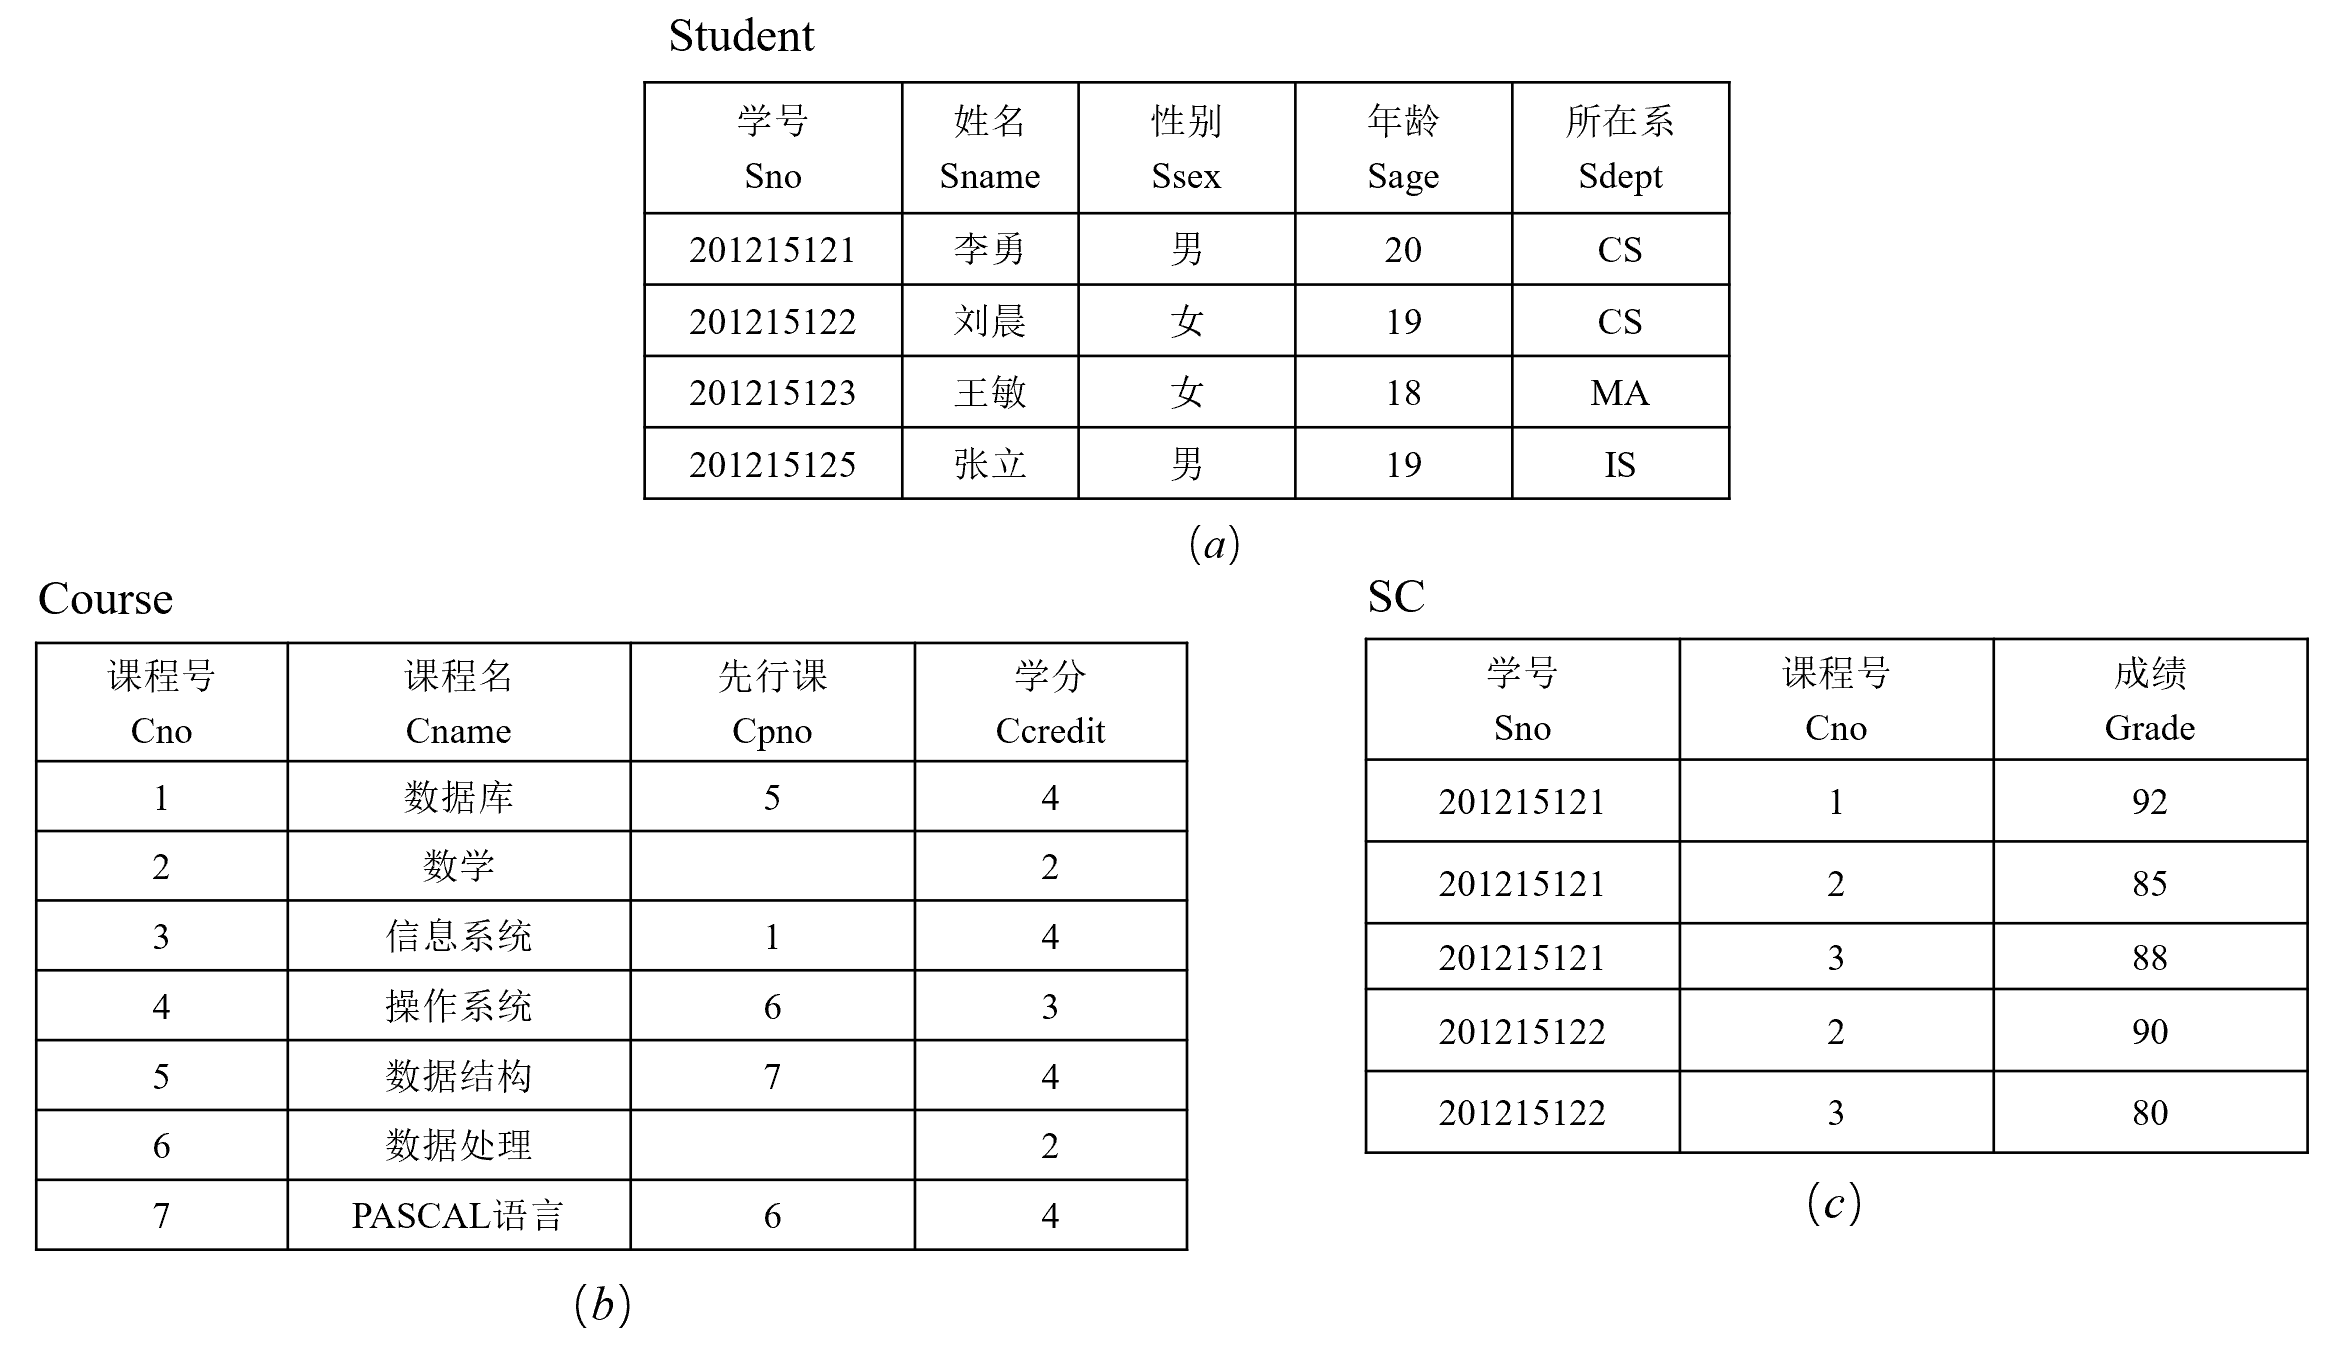
\includegraphics[width=0.95\textwidth]{images/2.3.2}
    \vspace{-1em}
\end{figure}

\subsubsection{选择}
\begin{itemize}
    \item 选择又称为限制
    \item 选择是在关系 $R$ 中选择满足给定条件的诸元组,记作
    $$\sigma_F (R)=\{t|t\in R \wedge F(t) = \mbox{“真”}\}$$
    其中 $F$ 表示选择条件,它是一个逻辑表达式,取逻辑值“真”或“假”
    \begin{itemize}
        \item 逻辑表达式 $F$ 的基本形式为 $X_1 \uptheta Y_1$,其中 $\uptheta$ 表示比较运算符。在基本的选择条件上可以进一步进行逻辑运算
    \end{itemize}
    \item 选择运算是从行角度进行的运算
\end{itemize}

例:查询信息系(IS系)全体学生:$\sigma _{\mathrm{Sdept='IS'}(\mathrm{Student})}$,结果如下:
\begin{table}[H]
    \centering
    \vspace{-0.5em}
    \begin{tabular}{|c|c|c|c|c|}
    \hline
    Sno       & Same & Sex & Sage & Slept \\\hline
    201215125 & 张立   & 男   & 19   & IS    \\\hline
    \end{tabular}
    \vspace{-1em}
\end{table}

\subsubsection{投影}
\begin{itemize}
    \item 投影是从 $R$ 中选择出若干属性列组成新的关系,记作
    $$\Pi_A(R) = \{t[A]| t \in R\}$$
    \item 投影操作主要是从列的角度进行运算
    \item 投影之后不仅取消了原关系中的某些列,而且还可能取消某些元组(避免重复行)
\end{itemize}

例:查询学生关系 $\mathrm{Student}$ 中都有哪些系,即查询关系 $\mathrm{Student}$ 上所在系属性上的投影:$\Pi _\mathrm{Sdept}(\mathrm{Student})$,结果如下:
\begin{table}[H]
    \centering
    \vspace{-0.5em}
    \begin{tabular}{|c|}
        \hline
        Sdept \\ \hline
        CS    \\ \hline
        IS    \\ \hline
        MA    \\ \hline
    \end{tabular}
    \vspace{-1em}
\end{table}

\subsubsection{连接}
\begin{itemize}
    \item 连接也称为 $\uptheta$ 连接,是从两个关系的笛卡尔积中选取属性间满足一定条件的元组,记作
    $$R \bowtie S =\{\overset{\frown}{t_rt_s} |t_r \in R \wedge t_s \in S \wedge t_r[A]\uptheta t_s[B]\}$$
    \item 连接运算从 $R$ 和 $S$ 的广义笛卡尔积 $R\times S$ 中选取 $R$ 关系在 $A$ 属性组上的值与 $S$ 关系在 $B$ 属性组上的值满足比较关系 $\uptheta$ 的元组
    \item 连接运算中最为重要且最为常用的连接为等值连接和自然连接
    \begin{itemize}
        \item $\uptheta$ 为“$=$”的连接运算称为等值连接
        \begin{itemize}
            \item 是从关系 $R$ 与 $S$ 的广义笛卡尔积中选取 $A,B$​ 属性值相等的那些元组,即等值连接为:
            $$R \mathop\bowtie \limits_{A=B} S =\{\overset{\frown}{t_rt_s} |t_r \in R \wedge t_s \in S \wedge t_r[A]= t_s[B]\}$$
        \end{itemize}
        \item 自然连接是一种特殊的等值连接
        \begin{itemize}
            \item 要求两个关系中进行比较的分量必须是相同的属性组
            \item 并且在结果中把重复的属性列去掉
            \item 若 $R$ 和 $S$ 具有相同的属性组 $B$,$U$ 为 $R$ 和 $S$​ 的全体属性集合,则自然连接可记作
            $$R \bowtie S =\{\overset{\frown}{t_rt_s}[U-B] |t_r \in R \wedge t_s \in S \wedge t_r[B]= t_s[B]\}$$
        \end{itemize}
        \item 一般的连接操作是从行的角度进行运算
        \item 自然连接还需要取消重复列,所以是同时从行和列的角度进行运算。
    \end{itemize}
\end{itemize}

例:设下图 $(a)$ 和 $(b)$ 分别为关系 $R$ 和关系 $S$,图 $(c)$ 为非等值连接 $R \mathop\bowtie \limits_{C<E} S$ 的结果,图 $(d)$ 为等值连接$R \mathop\bowtie \limits_{R.B=S.B} S$ 的结果,图 $(e)$ 为自然连接 $R \bowtie S$ 的结果
\begin{figure}[H]
    \vspace{-0.5em}
	\centering
	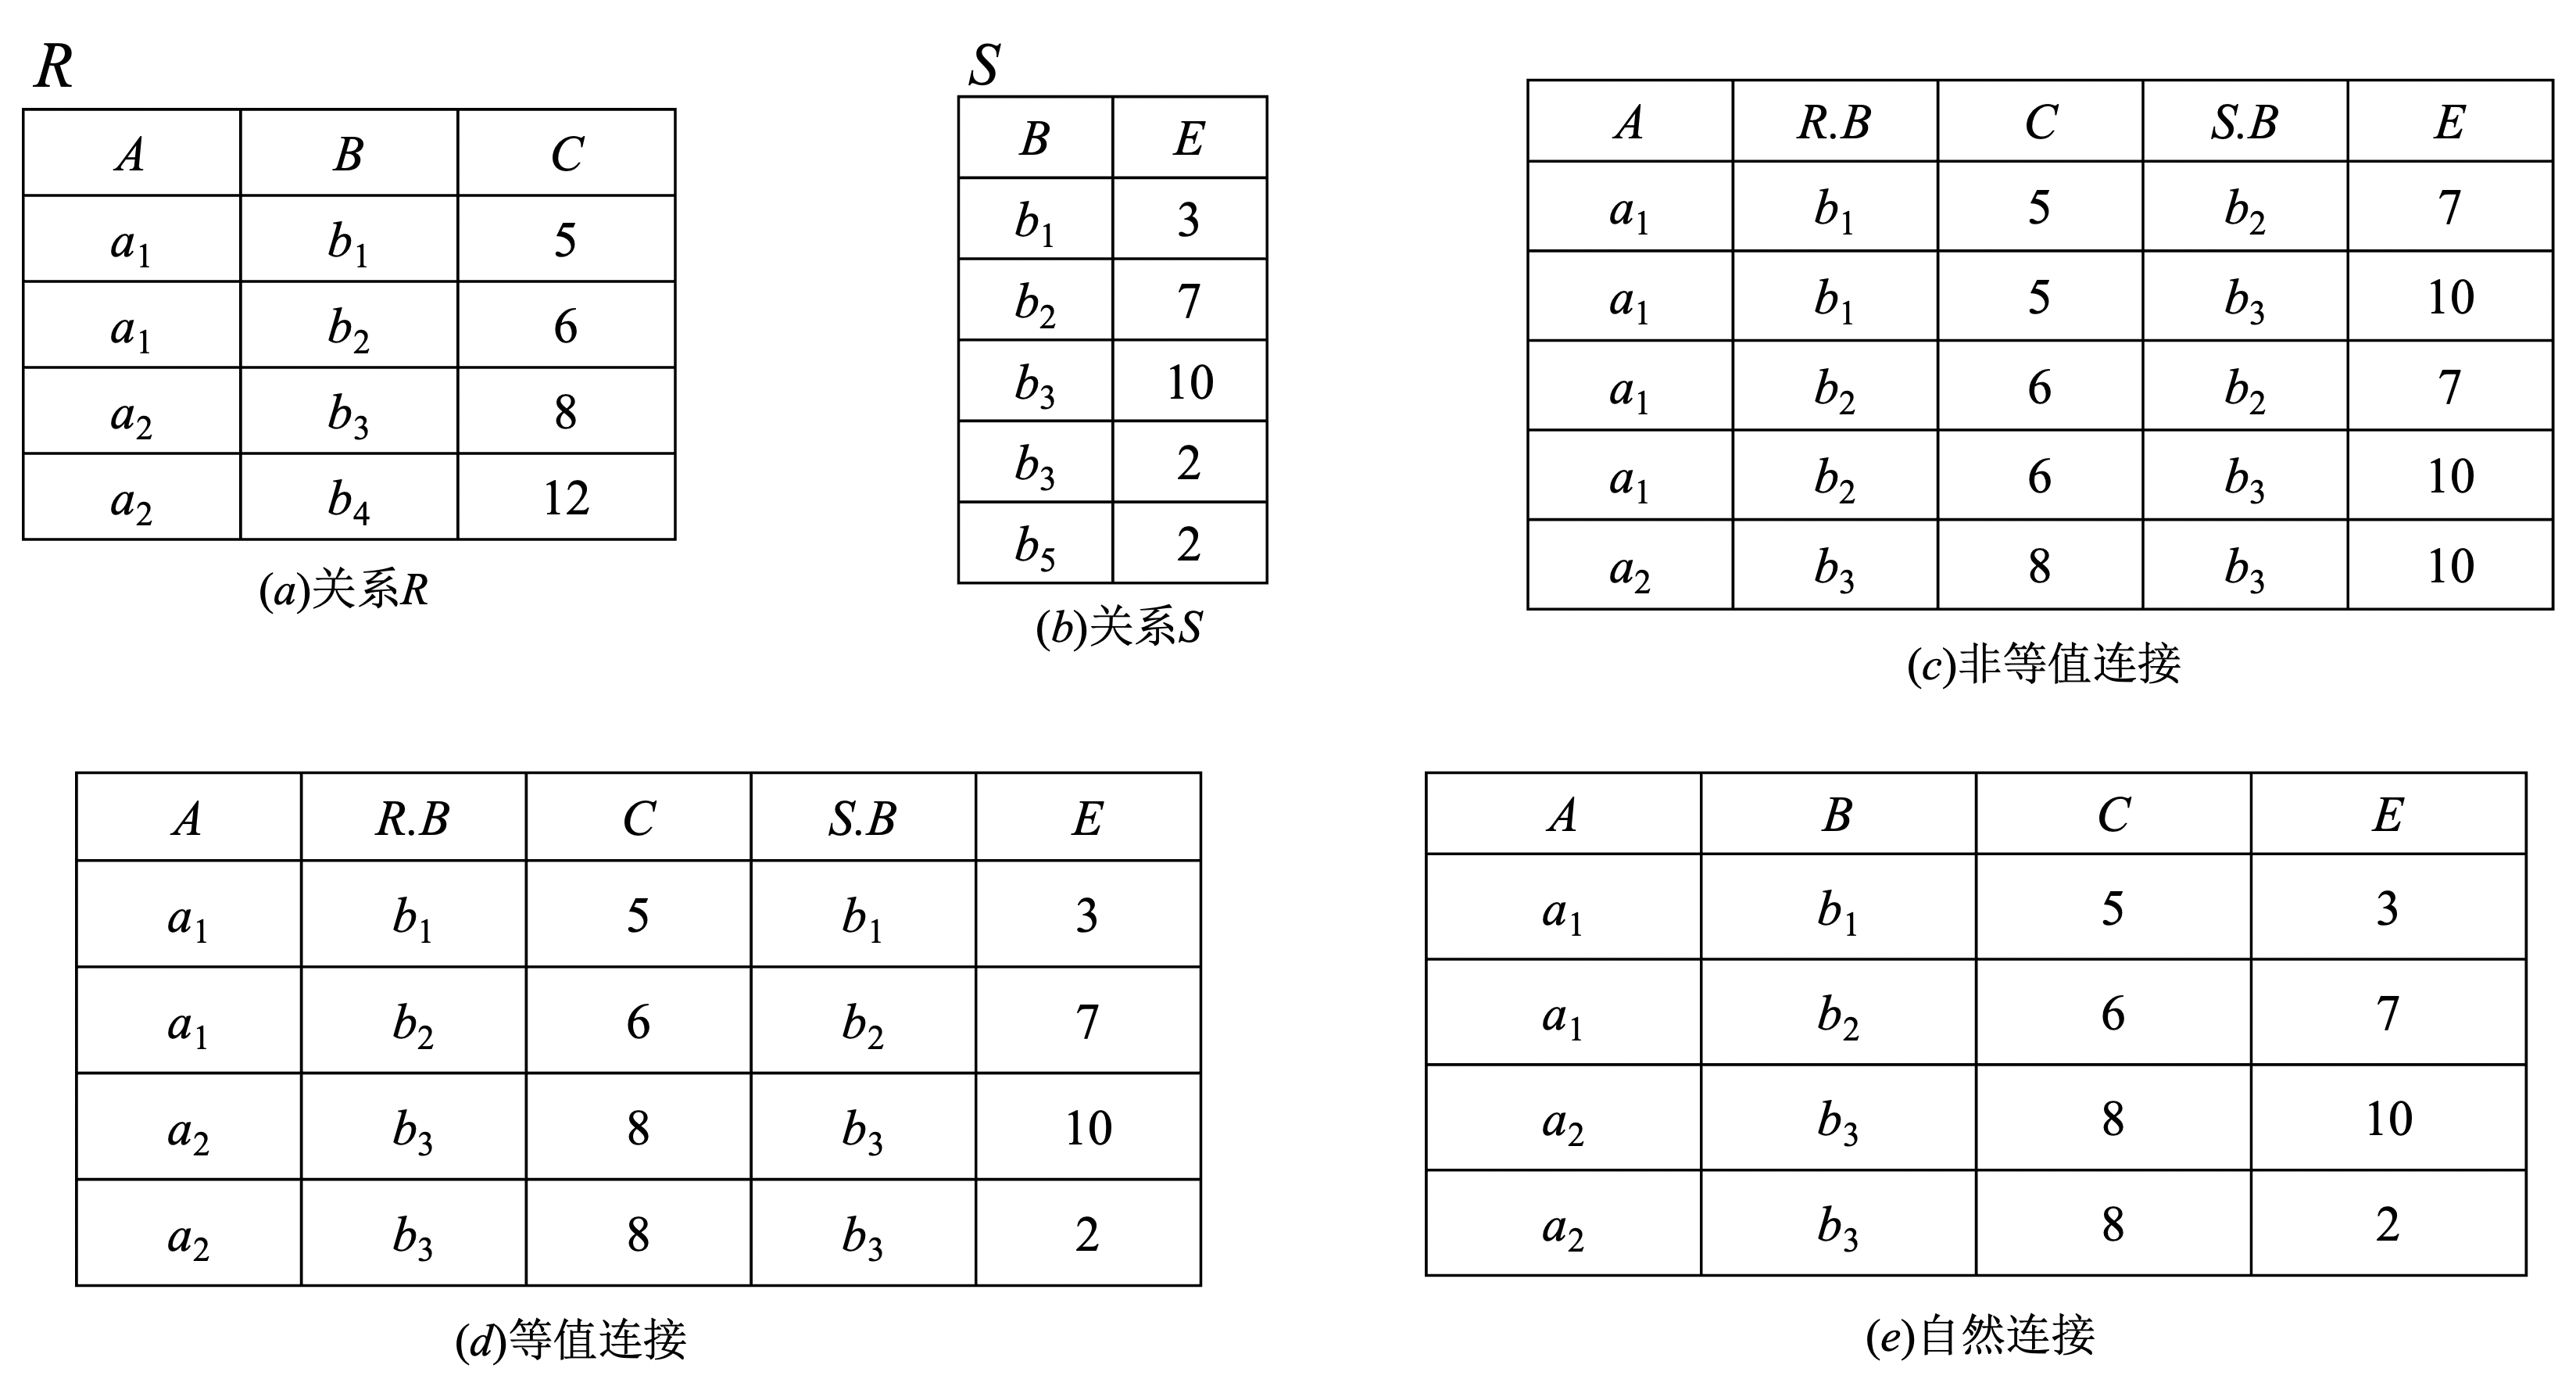
\includegraphics[width=0.95\textwidth]{images/2.3.3.3.1}
    \vspace{-1em}
\end{figure}

\begin{itemize}
    \item 两个关系 $R$ 和$S$ 在做自然连接时,关系 $R$ 中某些元组有可能在 $S$ 中不存在公共属性上值相等的元组,从而造成 $R$ 中这些元组在操作时被舍弃了,这些被舍弃的元组称为\textbf{悬浮元组}
    \item 如果把悬浮元组也保存在结果关系中,而在其他属性上填空值(Null),就叫做\textbf{外连接},记作 
\includegraphics[scale=1]{images/full outer join.pdf}
    \begin{itemize}
        \item 如果只保留左边关系 $R$ 中的悬浮元组,则称为\textbf{左外连接},记作
        
\includegraphics[scale=1]{images/left outer join.pdf}
        \item 如果只保留右边关系 $S$ 中的悬浮元组,则称为\textbf{右外连接},记作
        
\includegraphics[scale=1]{images/right outer join.pdf}
    \end{itemize}
\end{itemize}

例:下图 $(a)$ 是上例中关系 $R$ 和关系 $S$ 的外连接,图 $(b)$ 是左外连接,图 $(c)$ 是右外连接
\begin{figure}[H]
    \vspace{-0.5em}
	\centering
	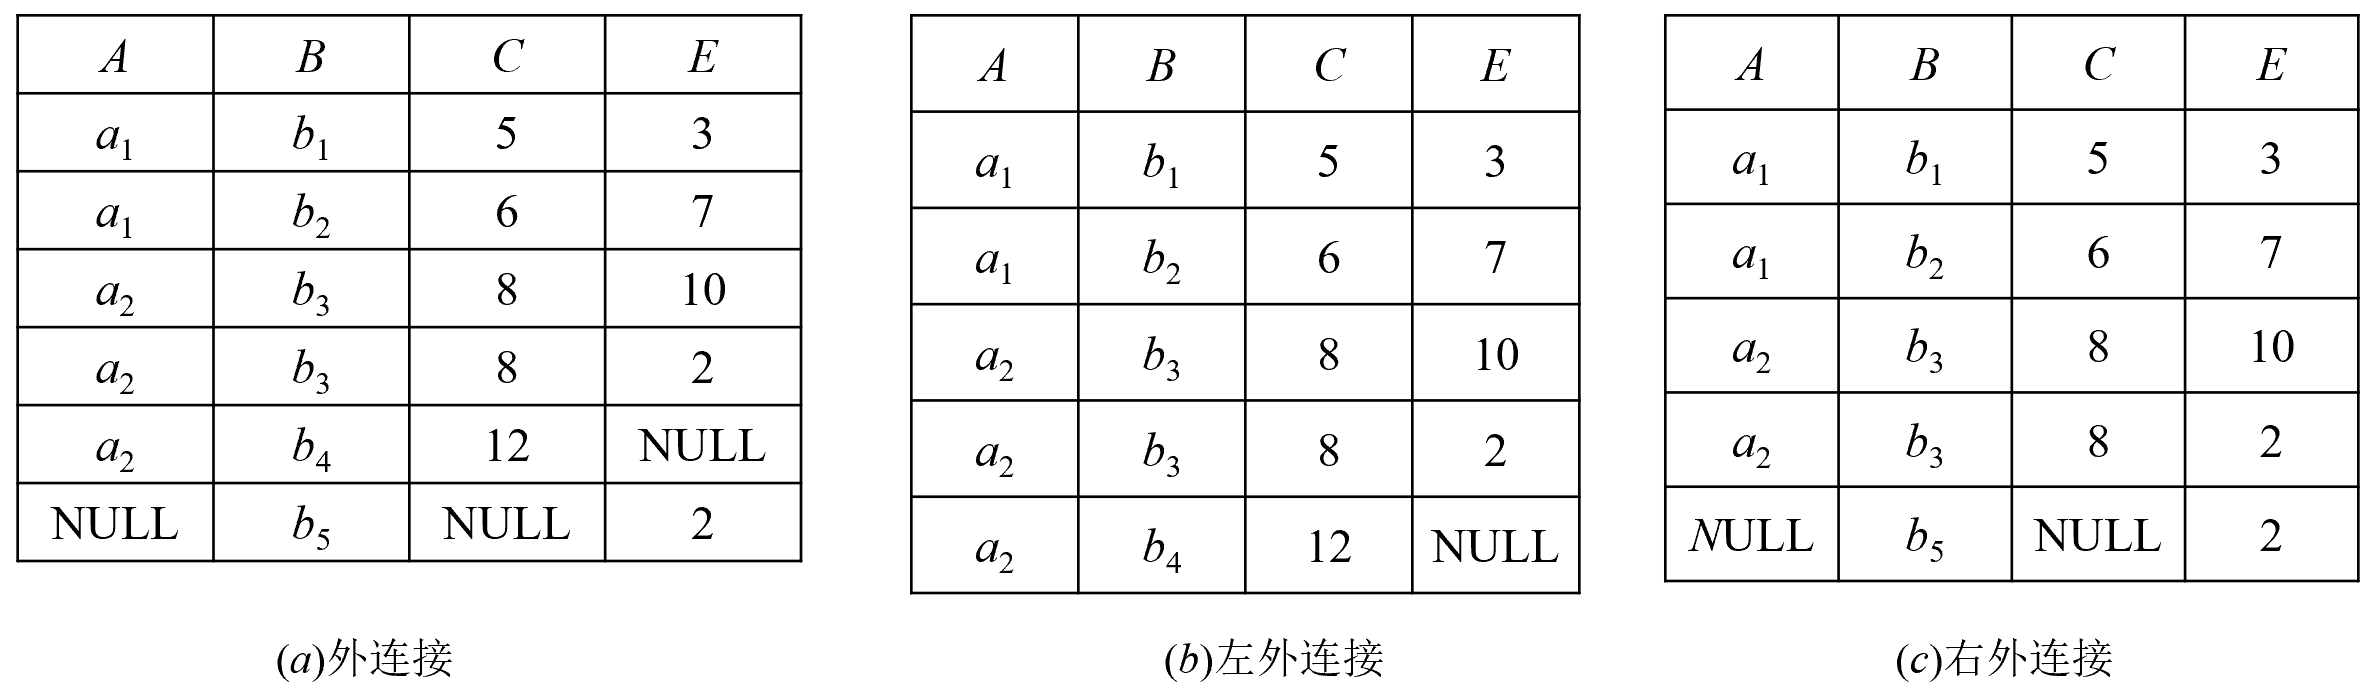
\includegraphics[width=0.8\textwidth]{images/2.3.3.3.2}
    \vspace{-1em}
\end{figure}

\subsubsection{除运算}
设关系 $R$ 除以关系 $S$ 的结果为关系 $T$,则 $T$ 包含所有在 $R$ 但不在 $S$ 中的属性及其值,且 $T$ 的元组与 $S$ 的元组的所有组合都在 $R$ 中

用\textbf{象集}定义除运算:
\begin{itemize}
    \item 给定关系 $R(X,Y)$ 和 $S(Y,Z)$,其中 $X,Y,Z$ 为属性组
    \item $R$ 中的 $Y$ 与 $S$ 中的 $Y$ 可以有不同的属性名,但必须出自相同的域集
    \item $R$ 与 $S$ 的除运算得到一个新的关系 $P(X)$,$P$ 是 $R$ 中满足下列条件的元组在 $X$ 属性列上的投影:元组在 $X$ 上分量值 $x$ 的象集 $Y_x$ 包含 $S$ 在 $Y$ 上投影的集合,记作:
    $$R\div S =\{t_r[X] |t_r\in R \wedge \Pi_Y(S) \subset Y_X\}$$
    其中 $Y_x$ 为 $x$ 在 $R$ 中的象集,$x=t_r[X]$
    \item 除是同时从行和列的角度进行运算
\end{itemize}

例:设关系 $R,S$ 分别为下图中的 $(a)$ 和 $(b)$ ,$R\div S$ 的结果如图 $(c)$
\begin{figure}[H]
    \vspace{-0.5em}
	\centering
	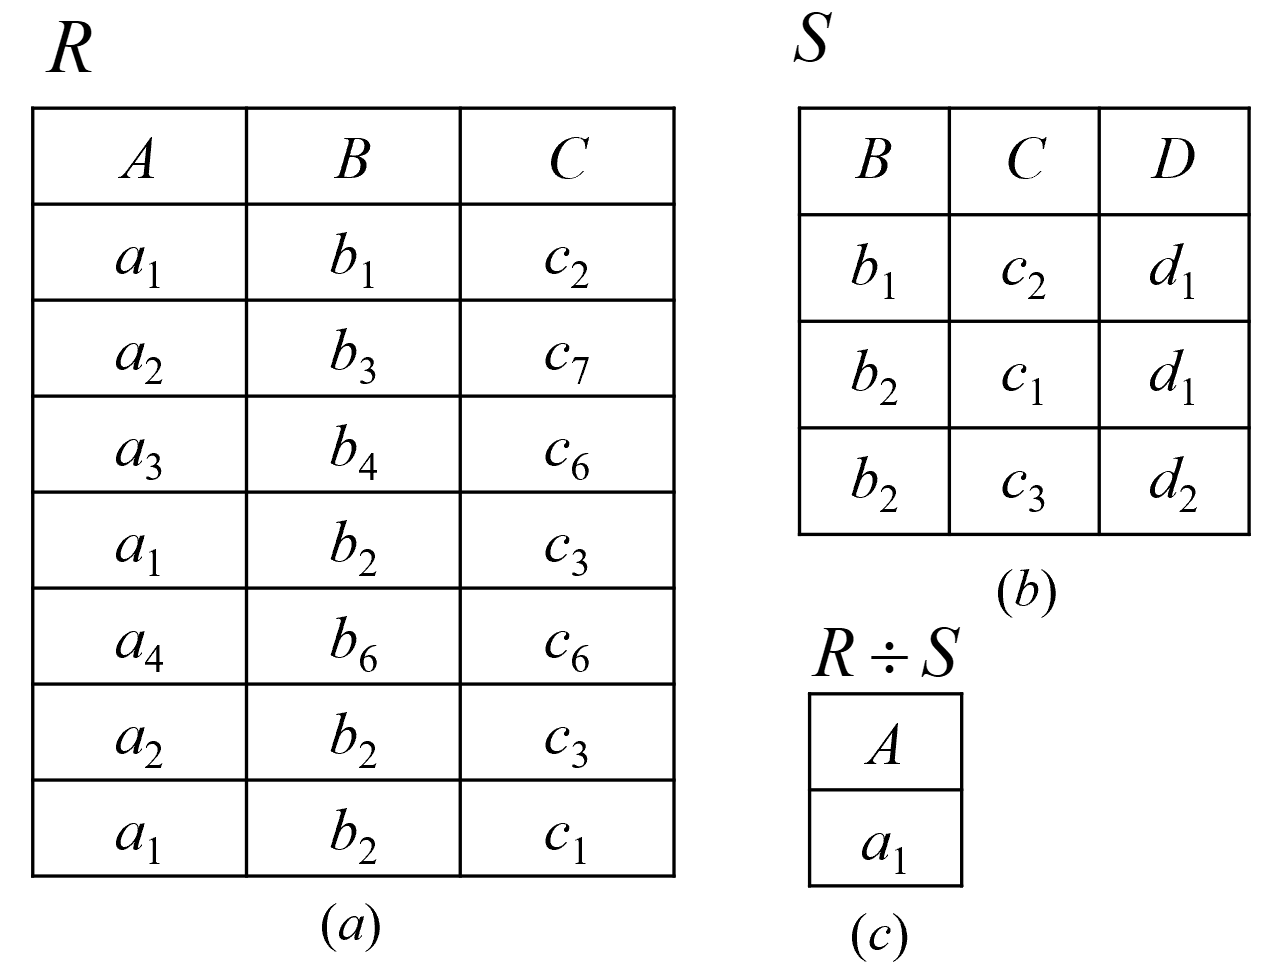
\includegraphics[width=0.4\textwidth]{images/2.3.3.4}
    \vspace{-1em}
\end{figure}
	
	% \begin{figure}[H]
    % \vspace{-0.5em}
	% \centering
	% \includegraphics[width=0.4\textwidth]{images/}
    % \vspace{-1em}
	% \end{figure}

	% \vspace{-0.5em}
	
	% \begin{multicols}{2}
    % \begin{itemize}
    %     \item 
    % \end{itemize}
	% \end{multicols}
	% \vspace{-1em}


\end{document}


